\hypertarget{introduction}{%
\section{Introduction}\label{introduction}}

Fault-injection schedulers determine which behaviors a test can observe.
A scheduler may choose one communication partition for a protocol view,
one directed admission bit per peer pair, or distinct decisions for
different voting phases. Twins, randomized Byzantine testing, Netrix,
and ByzzBench demonstrate the practical value of controlled execution
\cite{bano2021twins,winter2023randomized,dragoi2024netrix,louroneto2025byzzbench}.
Their capabilities also make a semantic question unavoidable: when does
aggregating admission decisions preserve a safety counterexample?

Consider an enabling prevote and a later precommit carrying repair
evidence. They share a directed peer connection and a protocol round. A
phase-sensitive policy can admit the former and suppress the latter. An
admission bit fixed across both phases admits both or neither. Admitting
more evidence may change a validator's state before it issues a vote
needed by a conflicting quorum. Thus counting possible schedules does
not establish preservation of the observations that matter to a safety
test.

The critical boundary is \textbf{vote issuance}. If a repair message
arrives after an indispensable conflicting precommit has been signed, it
cannot remove that precommit from another validator's future
certificate. Repair before the second \emph{decision} can therefore be
too late. We call the collection of second-vote opportunities a
\textbf{repair frontier} and study which pivotal contributions can
jointly survive across it.

The one-pivot example is useful but does not characterize broader
scheduler domains. With several initially ready pivots, a coarse policy
can assign different validators to the two branches. With individual
vote deadlines, a repair may be movable on its own but incompatible with
delaying another repair. We connect these two effects. A graph derived
from a finite opportunity partial order describes the compatible sets of
unrepaired contributors; quorum deficits determine how large such a set
must be.

\hypertarget{contributions-and-scope}{%
\subsection{Contributions and scope}\label{contributions-and-scope}}

The main contribution is an exact scheduler characterization for an
explicit independent-pivot certificate schema. If there are \(k\)
unit-weight pivots, the two quorums need \(d_0,d_1\) pivotal
contributions, and \(\alpha(H)\) is the largest jointly reusable pivot
set in the derived repair graph, a coarse unsafe execution exists
exactly when

\[
\max(d_0,d_1)\le k,
\qquad d_0+d_1\le k+\alpha(H).
\]

This yields the exact minimum number of independently phase-split
channels required to recover a witness, a weighted extension, and a
precise account of how relaxing delivery order changes the result. The
graph reversal argument and its underlying optimization are classical;
the contribution is their connection to admission coupling, persistent
signed outputs, and quorum requirements.

We also repair the one-pivot criterion by stating persistence, enabling
necessity, observation coverage, and the correct repair deadline
explicitly. A complete four-validator execution realizes the mechanism
using guarded Tendermint-style transitions under one omitted round-0
lock update. It includes actual signed vote sets, nil votes, legal
timeout transitions, and a late-repair control whose two conflicting
decisions occur at unmutated validators. Exhaustive finite checks and a
scoped Lean development accompany these results.

The claims concern finite agreement observations and declared scheduling
domains. The four-validator model is derived from pinned CometBFT rules;
it does not execute the production client. The multi-pivot graph theorem
assumes independent behavioral contracts and complete coverage of the
stated opportunity orders. No universal ordering of test frameworks,
unbounded completeness, liveness result, or deployed-client
vulnerability follows.

\hypertarget{executions-observations-and-scheduling-domains}{%
\section{Executions, observations, and scheduling
domains}\label{executions-observations-and-scheduling-domains}}

A protocol is a labelled transition system
\(P=(S,s_0,M,A,\delta,\mathsf{emit})\). A delivery consumes an existing
emitted envelope

\[
m=(\mathit{id},v,\lambda,s,r,\mathit{payload}).
\]

Here \(v\) is the policy's view key, \(\lambda\) its phase label, and
\(s,r\) the \textbf{transport endpoints}. A signed message's author need
not be its current transport sender: gossip may relay an unchanged
authenticated vote. The bounded model distinguishes these fields and
counts certificate support by signer identity.

For a legal finite execution \(\tau\), let
\(O(\operatorname{last}(\tau))\) record decisions at the designated
correct observers. The state predicate \(\mathsf{Unsafe}\) means that
these observers have decided conflicting values. Define

\[
\mathsf{UnsafeObs}_G(P,\mathcal B)=
\{O(\operatorname{last}(\tau)):\tau\in L_G(P,\mathcal B),\
\mathsf{Unsafe}(\operatorname{last}(\tau))\}.
\]

Our separation claims compare emptiness of these sets. They do not
assert equality of every unsafe observation or preservation of a
particular fine trace.

A phase-sensitive policy has bits \(A_T(v,\lambda,s,r)\). A coarse
policy has bits \(A_D(v,s,r)\). Phase erasure opens an edge if any phase
was admitted:

\[
C_{\mathrm{type}}(A_T)(v,s,r)=\bigvee_\lambda A_T(v,\lambda,s,r).
\]

Admission is only one part of a scheduler. The domain \(\mathcal B\)
also specifies message generation, event opportunities, ordering,
pending messages, and termination. The original fixed-order domain uses
a stable admission filter and predetermined delivery points. Later
sections admit all linear extensions of an explicitly stated partial
order. A directed graph by itself implies neither FIFO delivery nor an
obligation to process repair before a given vote.

\hypertarget{a-standard-sufficient-preservation-condition}{%
\subsection{A standard sufficient preservation
condition}\label{a-standard-sufficient-preservation-condition}}

The useful positive baseline is a specialized simulation argument
\cite{lynch1995simulations}. Let a candidate coarse trace retain the
actions of a fine trace in order and insert closure-required deliveries.
Suppose a preorder \(\mathcal R\) relates the initial states, each
insertion increases the target state in \(\mathcal R\), retained actions
preserve \(\mathcal R\), and unsafety is upward closed in
\(\mathcal R\).

\textbf{Theorem 1 (legal relational preservation).} If the candidate
trace \(C(\tau)\) is legal in the coarse language,
\(C(\tau)\in L_{G_D}(P,\mathcal B)\), these conditions imply
\(\mathsf{Unsafe}(\operatorname{last}(\tau))\Rightarrow \mathsf{Unsafe}(\operatorname{last}(C(\tau)))\).

\textbf{Proof.} Induct over the merged action sequence. At an insertion,
the target's increasing step composes with the current relation by
transitivity. At a retained action, forward simulation advances both
states. The terminal relation and upward closure transfer unsafety.
Target legality supplies membership in the coarse execution language.
\(\square\)

Legality is an independent obligation. Processing repair may disable an
action or prevent a message from being emitted, so simply retaining all
fine votes after inserting repair can produce an illegal sequence. Our
negative results instead rerun guarded opportunities; a disabled
opportunity emits no vote. Theorem 1 is supporting machinery, not a new
general simulation principle.

\hypertarget{a-corrected-one-pivot-separation-criterion}{%
\section{A corrected one-pivot separation
criterion}\label{a-corrected-one-pivot-separation-criterion}}

Let \(q\ge1\) be a certificate threshold. Two conflicting certificate
families have fixed nonpivot support \(q-1\) each. The same pivot \(p\)
is the only possible additional signer. The first and second votes are
issued at opportunities \(V_0,V_1\); \(C_0,C_1\) collect their
certificates. Decisions, signed votes, and the availability of emitted
votes at the specified collectors are irreversible within the bound.

The following are \textbf{behavioral obligations}:

\begin{enumerate}
\def\labelenumi{\arabic{enumi}.}
\tightlist
\item
  \textbf{Enabling necessity.} The first pivotal vote is emitted exactly
  when the enabling envelope \(E\) is admitted. No substitute supplies
  that missing contribution.
\item
  \textbf{Explicit persistence.} When \(E\) is admitted and repair \(R\)
  is withheld, \(p\) emits the second pivotal vote at \(V_1\). Other
  fixed events do not independently disable it.
\item
  \textbf{Timely repair.} When \(E,R\) are admitted and \(R\) is
  processed before \(V_1\), \(p\) does not emit the second pivotal vote.
  No previously emitted second-family signature can substitute for it.
\item
  \textbf{Certificate and observation coverage.} The two designated
  correct observers decide their respective values exactly when the
  corresponding quorum is available; the bounded agreement observation
  is unsafe exactly when both families decide. No unrelated decision
  opportunity creates an additional disagreement.
\end{enumerate}

The \textbf{scheduler obligations} are separate: \(E,R\) are emitted,
share one endpoint/view key, and have distinct phase labels. Fine
admission can realize \((e,r)=(1,0)\); coarse admission realizes only
\((0,0)\) and \((1,1)\). The relevant order is

\[
E<V_0<C_0<R<V_1<C_1.
\]

All other delivery choices and opportunities are fixed, and each rerun
obeys the behavioral guards. These assumptions deliberately describe a
sufficient schema; quorum arithmetic alone cannot establish a protocol
refinement.

\textbf{Theorem 2 (behavioral quorum-pivot separation).} Under these
behavioral and scheduler obligations,

\[
\mathsf{UnsafeObs}_{G_T}(P,\mathcal B)\ne\varnothing,
\qquad
\mathsf{UnsafeObs}_{G_D}(P,\mathcal B)=\varnothing.
\]

\textbf{Proof.} Fine admission supplies the first vote by enabling
necessity and the second by explicit persistence. Each augments a base
of \(q-1\), producing two conflicting correct decisions. With the coarse
edge off, the first vote is absent and its certificate is short,
regardless of whether \(p\) can still vote second. With the edge on, the
first certificate forms but timely repair prevents the second pivotal
signature. Observation coverage makes these two coarse cases exhaustive
for agreement. \(\square\)

The persistence obligation cannot be inferred from the absence of \(R\).
For example, a fixed local transition after \(C_0\) could disable \(p\)
even when \(R\) is suppressed. The endpoint and quorum conditions would
still hold, but the fine witness would disappear. Likewise, the order
\(R<C_1\) is insufficient if \(V_1<R<C_1\): repair cannot retract the
already signed vote. Both errors disappear when behavior and signature
timing are stated explicitly.

\hypertarget{the-original-quorum-family-and-its-extension}{%
\subsection{The original quorum family and its
extension}\label{the-original-quorum-family-and-its-extension}}

For every \(f\ge1\), take \(n=3f+1\), \(q=2f+1\), Byzantine set \(B\) of
size \(f\), correct exclusive sets \(A,C\) of size \(f\), and pivot
\(p\). Then

\[
Q_0=B\cup A\cup\{p\},\qquad Q_1=B\cup C\cup\{p\}
\]

have size \(q\) and each nonpivot base has size \(q-1\). Under the
behavioral contract, Theorem 2 applies. This arithmetic does not assert
that every locking protocol realizes the contract.

More generally, for \(1\le k\le f\), use \(k\) pivots, exclusive sets
\(A,C\) of size \(f+1-k\), Byzantine set \(B\) of size \(f\), and
\(k-1\) unused correct identities. The total is still \(3f+1\). Both
quorums contain \(B\), their exclusive set, and all \(k\) pivots; each
base has size \(q-k\). Distinct correct observers exist in nonempty
\(A,C\). The next theorem characterizes precisely which opportunity
orders can preserve these \(k\) required double contributions. The
extension is a certificate schema; the concrete protocol trace below
establishes the single-pivot case.

\hypertarget{repair-frontiers-for-several-independent-channels}{%
\section{Repair frontiers for several independent
channels}\label{repair-frontiers-for-several-independent-channels}}

Let \(I=\{1,\ldots,k\}\) be pivotal identities, each with positive
integer weight \(w_i\). Write \(w(X)=\sum_{i\in X}w_i\) and \(W=w(I)\).
The two certificate families have fixed base weights \(b_a\), thresholds
\(q_a\), and deficits \(d_a=\max(0,q_a-b_a)\), for \(a\in\{0,1\}\). Unit
weights give \(W=k\).

\hypertarget{behavioral-and-order-contracts}{%
\subsection{Behavioral and order
contracts}\label{behavioral-and-order-contracts}}

An admitted \(E_i\) enables exactly one first-family signature from
pivot \(i\). Once the first family is feasible, pivot \(i\) emits its
second-family signature at opportunity \(V_i\) \textbf{if and only if}
\(R_i\) has not been processed before \(V_i\). In particular, closing
its edge need not prevent its second vote: it was initially ready. No
other state transition changes this test. Admitted repair disables
prospective issuance; it cannot withdraw signed output. Both collectors
and the observation satisfy the coverage obligation of Section 3.

It suffices to impose this second-vote law on policies capable of
forming the first certificate. A policy that misses that certificate
cannot be unsafe in this two-family observation domain. This
qualification accommodates repairs whose commit evidence depends on
available first votes.

A finite strict partial order \(\prec\) describes opportunities,
including the fixed anchors

\[
E_i\prec V_0\prec C_0\prec V_i\prec C_1,
\qquad V_0\prec R_i.
\]

Additional relations specify the allowed delivery restrictions. Each
policy admits \textbf{all} linear extensions of this order, interpreted
through the guarded machine. Withheld deliveries and disabled voting
opportunities stutter. Their slots retain the stated precedence
constraints; suppression does not erase a transitive constraint between
other events. Every processed envelope must already be emitted and
available.

The \(k\) endpoint/view keys are independent. A coarse policy opens a
subset \(A\subseteq I\) and admits \(E_i,R_i\) together exactly for
\(i\in A\). Fine admission can admit all \(E_i\) and suppress all
\(R_i\). These are explicit independence and order-coverage assumptions.
If a real harness admits fewer orders, the model gives a sound
coarse-safety overapproximation, but an existential witness needs a
realizable order in that harness.

\hypertarget{a-graph-of-simultaneous-repair-obstructions}{%
\subsection{A graph of simultaneous repair
obstructions}\label{a-graph-of-simultaneous-repair-obstructions}}

Define a directed graph \(H\), including possible self-loops, by

\[
i\longrightarrow j \quad\Longleftrightarrow\quad R_i\prec V_j,
\qquad
\alpha(H)=\max\{|J|:J\subseteq I,\ H[J]\text{ is acyclic}\}.
\]

Use transitive precedence, not just a drawing's cover edges. A self-loop
means that a pivot's own repair is forced early.

\textbf{Lemma 1 (compatible late repairs).} For \(J\subseteq I\), a
linear extension can place \(V_i<R_i\) for every \(i\in J\) exactly when
\(H[J]\) is acyclic.

This is the standard reversible-pair/alternating-cycle argument from
partial-order theory, expressed in repair notation
\cite{streib2014dimension}. We include the proof because the mapping to
scheduling opportunities is central.

\textbf{Proof.} Add the required edges \(V_i\to R_i\) to the opportunity
order. Such an order exists exactly when the augmented relation is
acyclic: a finite acyclic relation has a topological ordering. A cycle
\(i_1\to\cdots\to i_t\to i_1\) in \(H[J]\) yields an augmented closed
walk

\[
V_{i_1}\to R_{i_1}\prec V_{i_2}\to R_{i_2}\prec\cdots\prec V_{i_1}.
\]

Conversely, any augmented cycle must use an added edge, since the
original order is acyclic. Between consecutive added edges
\(V_i\to R_i\) and \(V_j\to R_j\), the original-order segment gives
\(R_i\prec V_j\), hence \(i\to j\). Compress these segments to obtain a
nonempty closed walk in \(H[J]\), which contains a cycle. This includes
self-loops. \(\square\)

The graph can have cycles even though the opportunity order does not.
Its cycles describe incompatible \emph{requests to delay repair}, not a
causal cycle in an actual execution.

\hypertarget{exact-capacity-and-separation}{%
\subsection{Exact capacity and
separation}\label{exact-capacity-and-separation}}

\textbf{Theorem 3 (repair-frontier characterization).} Under the
contracts above, fine unsafety is feasible exactly when
\(d_0,d_1\le W\). Coarse unsafety is feasible exactly when there exist
\(J\subseteq A\subseteq I\) satisfying

\[
H[J]\text{ acyclic},\qquad w(A)\ge d_0,
\qquad w(I\setminus A)+w(J)\ge d_1. \tag{1}
\]

For unit weights this is equivalent to

\[
\mathsf{UnsafeObs}_{G_D}\ne\varnothing
\quad\Longleftrightarrow\quad
\max(d_0,d_1)\le k\ \land\ d_0+d_1\le k+\alpha(H). \tag{2}
\]

Consequently strict phase/coarse separation holds exactly when

\[
\boxed{\max(d_0,d_1)\le k\quad\land\quad
 d_0+d_1>k+\alpha(H).} \tag{3}
\]

\textbf{Proof.} Fine admission can supply all first and second
signatures by admitting every enabling envelope and suppressing every
repair. No branch can receive more than weight \(W\), proving its
characterization.

For a coarse unsafe execution, let \(A\) be its open keys and let \(J\)
be those open pivots whose second votes precede their repairs. The first
support is exactly \(w(A)\). Because the first certificate is feasible,
the second-vote contract applies: closed pivots remain ready and open
pivots contribute second exactly when in \(J\). Thus the second support
is \(w(I\setminus A)+w(J)\). The execution realizes their joint
lateness, so Lemma 1 gives acyclicity and establishes necessity of (1).

Conversely, choose \(A,J\) satisfying (1). Lemma 1 gives an order in
which every member of \(J\) signs before repair. Open precisely \(A\).
The first threshold is met, so the behavioral contract ensures second
signatures from every closed pivot and every member of \(J\). Further
signatures only increase support. Durable outputs reach both collectors;
observation coverage gives an unsafe execution.

For unit weights, adding \(d_0\le|A|\) and \(d_1\le k-|A|+|J|\) proves
the combined inequality in (2); each demand is at most \(k\). For the
converse put \(h=\max(0,d_0+d_1-k)\). Equation (2) implies
\(h\le\alpha(H)\) and \(h\le d_0\le k\). Choose an acyclic set of size
\(h\), possible by taking a subset of a maximum acyclic set, and extend
it to an open set \(A\) of size \(d_0\). Then \(k-|A|+h\ge d_1\), so (1)
applies. Combining fine feasibility with the negation of (2) gives (3).
\(\square\)

Here \(h\) is the number of pivots that must contribute to \textbf{both}
branches. Coarse reachability is decided by whether the scheduler can
keep that many jointly reusable contributors, not by the number of
admission bits alone.

\hypertarget{robustness-and-the-amount-of-phase-control-required}{%
\section{Robustness and the amount of phase control
required}\label{robustness-and-the-amount-of-phase-control-required}}

\hypertarget{common-deadlines-and-crossed-deadlines}{%
\subsection{Common deadlines and crossed
deadlines}\label{common-deadlines-and-crossed-deadlines}}

If all second signatures share one opportunity \(V\), let
\(F=\{i:R_i\prec V\}\) and \(\ell=k-|F|\). Members of \(F\) have
self-loops; all other pivots can jointly place repair after \(V\). Hence
\(\alpha(H)=\ell\) and (2) becomes \(d_0+d_1\le k+\ell\), subject to
individual feasibility. For the \(k\)-required family, \(d_0=d_1=k\):
separation survives whenever \(\ell<k\). Thus allowing some late repairs
need not eliminate separation once more than one double contribution is
indispensable.

Individual deadlines behave differently. With two pivots and only the
critical constraints

\[
R_1\prec V_2,\qquad R_2\prec V_1,
\]

each repair can individually follow its own vote. They cannot both do
so: that would require \(V_1<R_1<V_2<R_2<V_1\). The repair graph is a
directed two-cycle and \(\alpha(H)=1\), despite having no self-loop.
With \(d_0=d_1=2\), coarse admission remains safe and phase-sensitive
admission is unsafe. This is a separation over several event orders and
two independently controlled channels, rather than two executions of one
fixed edge.

\begin{figure}[t]
\centering
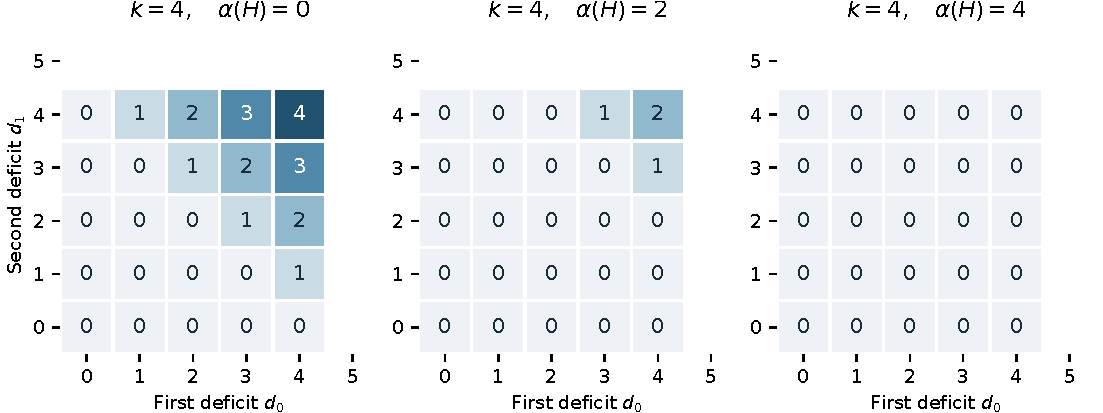
\includegraphics[width=0.96\textwidth]{../figures/repair_frontier_boundary.pdf}
\caption{Exact phase-control budget in the independent-pivot schema. Each cell is the minimum number of phase-split keys required to expose an unsafe witness. Blank cells exceed the available pivot count. Panels differ only in the capacity of jointly late repair, not in quorum size.}
\label{fig:frontier}
\end{figure}

\hypertarget{optimal-phase-splitting-budget}{%
\subsection{Optimal phase-splitting
budget}\label{optimal-phase-splitting-budget}}

A split key admits its enabling phase while suppressing repair.
Splitting leaves the opportunity partial order intact. With a chosen
split set \(T\), the maximum number of double contributors is

\[
|T|+\alpha(H[I\setminus T]).
\]

Among unsplit keys, Lemma 1 still applies. A split pivot contributes
twice without requiring its repair to be late. Choosing at most \(t\)
split keys gives the exact best capacity \(\min(k,\alpha(H)+t)\): this
is an upper bound because any unsplit acyclic set has size at most
\(\alpha(H)\); it is attained by keeping a maximum acyclic set and
splitting vertices outside it.

\textbf{Corollary 1 (minimum phase budget).} For unit weights, if fine
admission is feasible, the exact minimum number of independently split
keys needed for an unsafe witness is

\[
\boxed{t_* = \max(0,d_0+d_1-k-\alpha(H)).} \tag{4}
\]

\textbf{Proof.} Substitute the best capacity \(\min(k,\alpha(H)+t)\)
into (2). Since \(d_0,d_1\le k\), the resulting inequality holds exactly
when \(t\) covers the deficit in (4). \(\square\)

The statement is existential over the choice of split keys. It does not
claim that every set of \(t_*\) arbitrary message exceptions suffices. A
witness can be constructed by choosing an acyclic reusable set,
selecting the necessary split keys and open keys, adding its lateness
constraints, and topologically sorting the opportunity graph.

\hypertarget{order-relaxation-extra-edges-and-weights}{%
\subsection{Order relaxation, extra edges, and
weights}\label{order-relaxation-extra-edges-and-weights}}

Removing precedence constraints cannot add an edge to \(H\), so it
cannot decrease \(\alpha(H)\). Thus order relaxation weakens separation
monotonically under the same behavioral contract and deficits.
Conversely, additional causal paths may increase the needed phase
budget. Independent auxiliary events and extra edges are harmless only
if they preserve both relevant state/output behavior and the stated
order language. An extra substitute vote changes a deficit and must be
included in the calculation.

Initially ready and enabling-dependent pivots are different models. With
two forced-early pivots and deficits \(1,1\), coarse admission can open
one key for the first vote and close the other for the second. Requiring
both pivots to see enabling evidence before their second votes would
incorrectly remove that coarse witness. Theorem 3 uses the initially
ready behavior present in the four-validator edge-off case.

For a common deadline with integer weights, define \(L=I\setminus F\)
and \(W_L=w(L)\). The exact condition is existence of \(K\subseteq F\)
such that

\[
\max(0,d_0-W_L)\le w(K),\qquad w(K)+d_1\le W. \tag{5}
\]

Open every key in \(L\) and delay those repairs; choose \(K\) among the
forced-early keys. The two supports become \(W_L+w(K)\) and \(W-w(K)\).
Opening all \(L\) cannot hurt either branch, which proves necessity as
well as sufficiency. Indivisible weights matter: weights \(2,2\), no
late repair, and deficits \(1,3\) require an unattainable subset weight
\(1\). A total-weight relaxation would give the wrong answer. This is an
abstract weighted certificate result, not a weighted CometBFT
refinement.

For arbitrary individual deadlines, deciding whether a coarse unsafe
execution exists is NP-complete for explicitly represented finite
opportunity orders with unbounded \(k\). Appendix A gives the short
reduction using a classical graph construction
\cite{karp1972reducibility}; the contribution is the scheduler
correspondence, not a new graph-hardness result.

\hypertarget{a-complete-four-validator-tendermint-style-execution}{%
\section{A complete four-validator Tendermint-style
execution}\label{a-complete-four-validator-tendermint-style-execution}}

\hypertarget{source-mutation-and-transport}{%
\subsection{Source, mutation, and
transport}\label{source-mutation-and-transport}}

The new model uses CometBFT v0.39.3 at commit
\nolinkurl{49b82838fcca442b2445f76605c101609ed04130}
\cite{cometbft0393,cometbft0393code}. It follows the exercised proposal,
prevote, precommit, valid-block, timeout, and commit guards. A PoLC is a
locally received set of three matching prevotes; a commit certificate is
three matching precommits from distinct signers. The model has local
vote sets and explicit emitted envelopes, with no synthetic network
\texttt{POLKA} or \texttt{COMMIT} messages.

Take one height, equal weights, \(n=4,q=3\), Byzantine identity \(B\),
and protocol-following identities \(A,P,C\). Only \(P\)'s round-0
assignment of its persistent locked value and locked round is omitted in
the mutant; its valid-block update and its round-1 lock update execute
normally. The baseline omits nothing. The two reported conflicting
observers, \(A\) and \(C\), are unmutated. Calling \(P\)
protocol-following is relative to the explicitly mutated program, not a
claim that it follows the original locking specification.

Fix proposers \(B\) in round 0 and \(C\) in round 1. Initially every
correct replica is unlocked, with no valid block or decision. \(B\)
signs a block-0 proposal and sends it to \(A\), which relays the same
signed proposal and block to \(P\). Thus changing the controlled
\(B\to P\) edge does not secretly change proposal delivery. That edge's
round-0 envelopes are exactly

\[
E=B\!:\!\operatorname{PREVOTE}(0,0),\qquad
R=B\!:\!\operatorname{PRECOMMIT}(0,0),
\]

where arguments are \((\text{round},\text{block})\). Both are emitted
before \(E\) is attempted; \(B\) may sign adversarially. All other
peer/round admission outcomes are fixed and type-uniform. The complete
trace audits this property, distinguishes transport sender from signer,
and records suppressed or unavailable delivery opportunities.

\hypertarget{the-phase-sensitive-mutant-trace}{%
\subsection{The phase-sensitive mutant
trace}\label{the-phase-sensitive-mutant-trace}}

Write \(\operatorname{PV}(r,x)\) and \(\operatorname{PC}(r,x)\) for
height-1 prevotes and precommits; \(\bot\) denotes nil. Self-votes below
are actual emitted self-envelopes. Each local quorum is formed from
messages already received.

\begin{enumerate}
\def\labelenumi{\arabic{enumi}.}
\tightlist
\item
  \(A\) receives \(B\)'s block-0 proposal and signs
  \(\operatorname{PV}(0,0)\). \(A\) relays the proposal to \(P\), which
  signs the same prevote. \(C\) receives no proposal; its proposal
  timeout produces \(\operatorname{PV}(0,\bot)\).
\item
  \(B\) emits its round-0 prevote and precommit. Deliver \(P\)'s and
  \(B\)'s prevotes to \(A\). The set \(\{A,P,B\}:0\) makes \(A\) persist
  valid/locked block \(0@0\) and sign \(\operatorname{PC}(0,0)\).
\item
  Deliver \(A\)'s prevote and \(E\) to \(P\). Its same three-signer PoLC
  sets valid block \(0@0\). The mutation omits only its lock assignment,
  and \(P\) signs \(\operatorname{PC}(0,0)\) while remaining unlocked.
\item
  Deliver \(C\)'s nil prevote to \(P\), and the \(A,P\) block-0 prevotes
  to \(C\). At \(C\), the mixed set \(\{A:0,P:0,C:\bot\}\) enables its
  prevote timeout without creating a block-0 PoLC. On expiry, \(C\)
  signs \(\operatorname{PC}(0,\bot)\).
\item
  Deliver \(A\)'s precommit to \(P,C\), and \(P\)'s precommit to
  \(A,C\). Deliver \(B\)'s precommit to \(A\). Its local set
  \(\{A,P,B\}:0\) reaches three and \(A\) decides 0.
\item
  Deliver \(C\)'s nil precommit to \(P\). Both \(P\) and \(C\) now have
  the mixed set \(\{A:0,P:0,C:\bot\}\). It enables a precommit timeout
  but does not commit block 0. The fine policy suppresses \(R\). Expiry
  advances \(P,C\) lawfully to round 1.
\item
  \(P\) retains valid block \(0@0\) but no lock; \(C\) has neither.
  Consequently the unchanged proposer \(C\) can propose new block 1 with
  valid round \(-1\). \(C\) and the unlocked \(P\) each sign
  \(\operatorname{PV}(1,1)\). Making \(P\) the proposer instead would
  require accounting for its cached valid block 0.
\item
  \(B\) emits round-1 prevote and precommit for 1. Deliver the \(C,B\)
  prevotes to \(P\), producing PoLC \(\{P,C,B\}:1\). \(P\) normally
  updates valid/locked block to \(1@1\) and signs
  \(\operatorname{PC}(1,1)\). Deliver the \(P,B\) prevotes to \(C\); it
  obtains the same PoLC and precommits 1.
\item
  Deliver the \(P,B\) precommits to \(C\). Together with \(C\)'s
  self-precommit, they produce decision 1. Delivering the \(C,B\)
  precommits to \(P\) also lets it decide 1. The unmutated observers
  have \(A=0,C=1\).
\end{enumerate}

No unconditional jump between rounds is used. The mixed nil/block
precommit set is necessary to justify timeout-driven advancement without
giving \(P\) the block-0 commit. Nor is valid-block state silently
erased by the mutation. The artifact expands these nine groups into
every signature, envelope emission, reception, state change, and local
certificate.

\begin{table}[t]
\centering\small
\begin{tabular}{llcccc}
\toprule
Program & Round-0 admission & $A$ & $P$ & $C$ & Unsafe \\
\midrule
Baseline & $E$ only & 0 & -- & -- & no \\
Baseline & edge off & -- & 1 & 1 & no \\
Baseline & edge on & 0 & 0 & -- & no \\
Missing lock & $E$ only & 0 & 1 & 1 & yes \\
Missing lock & edge off & -- & 1 & 1 & no \\
Missing lock & edge on & 0 & 0 & -- & no \\
\bottomrule
\end{tabular}
\caption{Actual terminal decisions in the six canonical guarded executions. A dash means no decision in this finite prefix, not a liveness failure.}
\label{tab:canonical}
\end{table}

With the fine baseline, \(P\) retains its lock and prevotes 0 in round
1; the second value-1 quorum is absent. With the coarse edge off, \(P\)
lacks the PoLC-completing \(E\), receives a mixed prevote quorum, and
precommits nil. \(A\) therefore misses its first certificate; \(P,C\)
may still decide 1. With the edge on in the fixed order, \(R\) completes
\(P\)'s actual round-0 precommit quorum. It commits/advances before
issuing the required round-1 vote. These are different generated
executions, not a table filled with assumed pivot contributions.

\hypertarget{repair-before-the-decision-can-still-fail}{%
\subsection{Repair before the decision can still
fail}\label{repair-before-the-decision-can-still-fail}}

Keep the coarse edge on and move \(R\). If it arrives after \(P\)'s
round-1 prevote but before its precommit opportunity, the mutant remains
safe: that prevote alone cannot supply the third value-1 precommit. If
it arrives after \(P\) has issued \(\operatorname{PC}(1,1)\) but before
\(C\) decides, the observed decisions are

\[
A=0,\qquad P=0,\qquad C=1.
\]

The repair commits \(P\) to 0 and stops further signing at the height.
Its already emitted round-1 votes still reach \(C\). When \(P\) lacks
the block matching its old-round certificate, it explicitly obtains
block 0 from \(A\) before finalizing; the model does not treat a vote as
block data.

The direct version permits a round-1 \(B\to P\) prevote to overtake the
buffered round-0 repair on that connection. We report this non-FIFO
assumption. A separate gossip control obtains the same conflict with
FIFO-compatible admitted vote-envelope order: \(B\) sends its round-1
prevote to \(C\), which relays that unchanged signed vote to \(P\); the
direct \(B\to P\) copy follows \(R\). This changes the fixed gossip
skeleton and is reported separately. It demonstrates a stronger timing
counterexample without silently attributing arbitrary packet reordering
to a FIFO transport. Neither control is an execution of the production
P2P reactor.

\hypertarget{validation-and-assurance}{%
\section{Validation and assurance}\label{validation-and-assurance}}

The new experiments vary admission, event order, compatible late-repair
sets, phase exceptions, and weights. Their role is to falsify incorrect
encodings of the stated contracts. They do not estimate bug prevalence
across protocols.

\begin{table}[t]
\centering\small
\begin{tabular}{p{0.30\textwidth}p{0.34\textwidth}p{0.25\textwidth}}
\toprule
Check & Exhaustive or declared scope & Outcome \\
\midrule
Repair graphs & All 530 directed graphs, including loops, for $k=1,2,3$; 50,363 legal orders & 1,357,209 policy/split executions \\
Reachability and budget & All deficit pairs $0\ldots k+1$ for each graph & 13,074 checks each; no mismatch \\
Joint lateness & All requested reusable subsets in those graphs & 4,164 checks; no mismatch \\
General event precedence & All 219 labelled partial orders on two repairs and two vote opportunities, supplied as cover edges & Order-to-graph checks pass \\
Common frontier & $k=1\ldots8$, all forced-repair counts; barrier timing representatives & 174,250 executions; 2,636 boundary checks \\
Weighted common frontier & 258 domains with up to three pivots, weights in $\{1,2,3\}$; extremal late order and all admissions & 15,700 boundary checks \\
Concrete protocol trace & Six canonical and six timing/route controls & 12 legality audits pass \\
\bottomrule
\end{tabular}
\caption{Validation of the revised models. Graph realizations exhaust their legal orders. The common and weighted sweeps use the stated support-equivalent or extremal orders; they are not advertised as all event permutations.}
\label{tab:validation}
\end{table}

The graph oracle executes guarded events and preserves emitted
signatures; it does not derive its outcomes from the theorem's capacity
formula. Only afterward does the checker compare all observed support
pairs and minimum split costs with the predictions. The general-order
suite independently constructs transitive closure, supplies cover edges
to the implementation, and checks paths passing through suppressed
opportunity slots. The weighted sweep deliberately retains the
indivisible-weight counterexample.

The concrete trace has independent post-execution audits for prior
emission, once-only envelope delivery, authentication, distinct actual
signers, local certificate timing, signing guards, and quorum-enabled
timeouts. Negative controls reject fabricated envelopes, altered
authenticators, duplicate votes or deliveries, insufficient PoLC
evidence, and unjustified timeout transitions. The canonical mutant and
the late-repair mutant expose disagreement at \(A,C\), which contain no
injected lock defect.

\hypertarget{what-lean-checks}{%
\subsection{What Lean checks}\label{what-lean-checks}}

The primary project is pinned to Lean 4.33.0. The revision adds a
theorem over an \textbf{arbitrary behavioral contract} for Theorem 2,
explicitly assuming positive persistence and the observation contract
rather than defining the desired safety classification. It also checks
the arithmetic capacity equivalence, its strict-separation form, the
minimum split budget under its capacity contract, the weighted admission
interval, and a small output machine in which later repair preserves an
earlier signature. The build includes an axiom audit and independent
rechecking of the resulting kernel objects.

The graph reversal lemma, the graph-to-execution correspondence, and the
derivation of optimal graph capacity are proved in the paper and tested
by finite enumeration. They are \textbf{not} claimed to be fully
mechanized by the arithmetic Lean module. The concrete message trace is
executable validation, not a Lean proof of the CometBFT client.

Earlier Lean, SMT, certificate-kernel, Python, and Go checks remain
available. In particular, agreement of 384 Python/Go rows for
\(f=1,\ldots,64\) checks the previous Boolean model's encoding. The old
theorem named \texttt{bounded\_tendermint\_refines\_quorum\_pivot}
establishes matching terminal classifications, not a transition
refinement. Increasing \(f\) in that family is not independent
validation of many protocols. The revised claim ledger records this
distinction.

\hypertarget{related-work-and-the-novelty-boundary}{%
\section{Related work and the novelty
boundary}\label{related-work-and-the-novelty-boundary}}

\textbf{Communication closure.} Drăgoi et al.~compare asynchronous
executions with lossy synchronous executions under implementation
conditions and develop testing based on communication closure
\cite{dragoi2020communication}. Their communication rounds distinguish
send/receive/update steps, including different protocol phases. Our
operator additionally couples admission across such steps within one
view key. The counterexample therefore does not refute their
normalization theorem or the effectiveness of their tester; it
identifies an obligation for a further aggregation.

\textbf{Byzantine testing.} Twins already describes certificate arrivals
advancing a stale twin in its preferred-round mutation experiment; its
underlying network playground can also filter message types
\cite{bano2021twins}. Consequently neither certificate evidence
destroying an intended attack state nor phase-selective APIs are claimed
as new. Distinguish the published partition-scenario generator from the
full executor's capabilities. ByzzFuzz, Netrix, and ByzzBench supply
mutation, programmable testing, and controlled benchmark infrastructures
\cite{winter2023randomized,dragoi2024netrix,louroneto2025byzzbench}. Our
contribution concerns the safety-observation language of a declared
admission/order contract, not a capability ranking of those systems.

\textbf{Preservation and partial orders.} Simulation with internal
actions is established machinery \cite{lynch1995simulations}. The
inconsistent-labelling literature shows why action-oriented reduction
conditions must be connected carefully to state observations
\cite{neele2021labelling}; its operator differs from phase admission
closure. Reversibility of incomparable pairs is characterized by absence
of alternating cycles in classical partial-order theory
\cite{streib2014dimension}. Lemma 1 uses that argument, and the
induced-acyclic optimization and symmetric-graph hardness construction
are classical \cite{karp1972reducibility}. The result developed here
combines this order characterization with initial readiness,
irreversible vote issuance, and certificate deficits, yielding the exact
scheduler phase budget and a guarded BFT-rule witness.

The literature audit supports this specific positioning, not an
assertion that no equivalent result exists in all prior literature.
Replay congruence and the earlier seven-flag diagnostic are retained as
supplementary results in Appendix B; they do not carry the main novelty
claim.

\hypertarget{limitations-and-reproducibility}{%
\section{Limitations and
reproducibility}\label{limitations-and-reproducibility}}

The strongest mathematical statements are conditional on the
independent-pivot and complete opportunity-order contracts. New edges
that supply substitute support, policies that change message generation
beyond these contracts, changing validator sets, recovery, and
interdependent locking behavior require a new conformance argument. The
weighted result concerns indivisible certificate weights with fixed
membership. It is not a staking or dynamic-quorum theorem.

The concrete source pin is reproducible: the artifact contains exact
v0.39.3 files, verified Git blob identifiers and SHA-256 hashes. The
older source snapshot is correctly retained as v0.40.0. Authentication
in the local model uses deterministic test-only tags to enforce signer
and envelope integrity; production serialization, cryptographic
implementation, proposer-priority updates, block-part gossip, and the
full event loop are not modeled end to end. The supplied proposer prefix
and aggregate complete-block deliveries are explicit environmental
choices.

The public working artifact is available at
\url{https://github.com/galetaa/twins-scheduler}. The revision provides
a single command, \texttt{./reproduce\_revision.sh}, that runs the
existing checks, new guarded traces and frontier enumeration, the
integrated Lean build and axiom audit, and the revised LIPIcs build. Raw
JSON/CSV outcomes, source pins, proof-to-claim mappings, and manuscript
sources are included. The command fails on a mandatory check failure.
Reproduction dependencies are pinned by the existing project; build logs
record the actual tool versions used.

\hypertarget{conclusion}{%
\section{Conclusion}\label{conclusion}}

The effect of phase erasure depends on both admission coupling and the
latest opportunity at which repair can still prevent an indispensable
signature. A complete four-validator trace makes the distinction between
state repair and durable signed output concrete. For an explicit
multi-pivot schema, the derived repair graph and quorum deficits give an
exact characterization of coarse unsafe reachability and the minimum
phase-control budget. This turns a single fixed-order counterexample
into a quantitative account of when order relaxation and additional
independently controlled channels preserve or destroy separation.

\hypertarget{acknowledgments-and-ai-use-disclosure}{%
\subsection{Acknowledgments and AI-use
disclosure}\label{acknowledgments-and-ai-use-disclosure}}

An OpenAI language model assisted with research organization, literature
discovery, proof exploration, manuscript drafting, code generation, and
consistency checking. The authors retain responsibility for the
correctness, originality, citations, and experimental claims. The model
is not an author.
